\documentclass[letterpaper,12pt,fleqn]{article}
\usepackage{matharticle}
\usepackage{tikz}
\usetikzlibrary{positioning}
\usetikzlibrary{calc}
\usetikzlibrary{shapes.gates.logic.US}
\pagestyle{plain}
\begin{document}

\begin{center}
  \large
  Math-42 Sections 01, 02, 05

  \Large
  Homework \#2 Solutions
\end{center}

\subsection*{Problem}

A flip-flop or latch is a device the locks the binary value on its input to its output upon a clock pulse (a
transition from \(0\) to \(1\)):

\bigskip

\begin{center}
  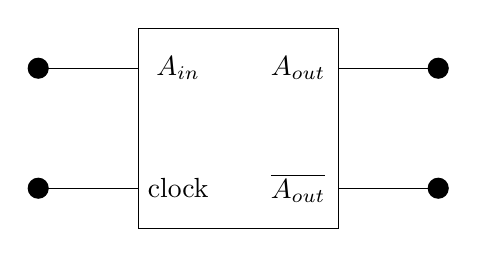
\begin{tikzpicture}
    \draw (0,0) rectangle (1in, 1in);
    \node at (0.2in, 0.8in) {\(A_{in}\)};
    \node at (0.2in, 0.2in) {clock};
    \node at (0.8in, 0.8in) {\(A_{out}\)};
    \node at (0.8in, 0.2in) {\(\overline{A_{out}}\)};
    \draw (-0.5in, 0.8in) -- (0in, 0.8in);
    \draw (-0.5in, 0.2in) -- (0in, 0.2in);
    \draw (1in, 0.8in) -- (1.5in, 0.8in);
    \draw (1in, 0.2in) -- (1.5in, 0.2in);
    \node [draw,circle,fill,inner sep=0in,minimum size=0.1in] at (-0.5in, 0.8in) {};
    \node [draw,circle,fill,inner sep=0in,minimum size=0.1in] at (-0.5in, 0.2in) {};
    \node [draw,circle,fill,inner sep=0in,minimum size=0.1in] at (1.5in, 0.8in) {};
    \node [draw,circle,fill,inner sep=0in,minimum size=0.1in] at (1.5in, 0.2in) {};
  \end{tikzpicture}
\end{center}

\bigskip

For example, if \(A_{out}=0\), \(A_{in}\) can vary between \(0\) and \(1\) but \(A_{out}\) will not change.  But if
\(A_{in}=1\) and a clock pulse is applied then \(A_{out}\) will change to \(1\) and will stay that way until a new
input value and clock pulse is applied.  Note that flip-flops usually provide both the latched value and its
negated value as outputs.

Your assignment is to use two flip-flops to design a binary counter from \(0\) to \(3\): \(00, 01, 10, 11, 00,
\ldots\).  Call the least significant bit \(A\) and the most significant bit \(B\).  Thus, the transitions should be
as follows:

\bigskip

\begin{center}
  \begin{tabular}{c|c}
    A & B \\
    \hline
    0 & 0 \\
    0 & 1 \\
    1 & 0 \\
    1 & 1 \\
    0 & 0
  \end{tabular}
\end{center}

\bigskip

The final complete circuit looks something like this:

\bigskip

\begin{center}
  \begin{tikzpicture}
    \draw (0in,0in) rectangle (1in, 1in);
    \node at (0.2in, 0.8in) {\(B_{in}\)};
    \node at (0.2in, 0.2in) {clock};
    \node at (0.8in, 0.8in) {\(B_{out}\)};
    \node at (0.8in, 0.2in) {\(\overline{B_{out}}\)};
    \draw (3in, 0in) rectangle (4in, 1in);
    \node at (3.2in, 0.8in) {\(A_{in}\)};
    \node at (3.2in, 0.2in) {clock};
    \node at (3.8in, 0.8in) {\(A_{out}\)};
    \node at (3.8in, 0.2in) {\(\overline{A_{out}}\)};
    \node at (2in, -1.5in) [draw,rectangle,minimum width=6in,minimum height=1in] {YOUR LOGIC CIRCUITS};
    \draw [<-] (0in, 0.8in) -| (-0.25in, -1in);
    \draw [<-] (3in, 0.8in) -| (2.75in, -1in);
    \draw [->] (1in, 0.2in) -| (1.25in, -1in);
    \draw [->] (1in, 0.8in) -| (1.5in, -1in);
    \draw [->] (4in, 0.2in) -| (4.25in, -1in);
    \draw [->] (4in, 0.8in) -| (4.5in, -1in);
    \draw (1.5in, 0.8in) -- (1.5in, 1.5in);
    \draw (4.5in, 0.8in) -- (4.5in, 1.5in);
    \node [draw,circle,fill,inner sep=0in,minimum size=0.1in] (B) at (1.5in, 1.5in) {};
    \node [draw,circle,fill,inner sep=0in,minimum size=0.1in] (A) at (4.5in, 1.5in) {};
    \node [above=1ex of A] {\(A\)};
    \node [above=1ex of B] {\(B\)};
  \end{tikzpicture}
\end{center}

\bigskip

You need to design the two logic circuits that take the outputs of the flip-flops as inputs to set up the proper
next values on the inputs so that the next sequence in the count is latched on the next clock pulse.  For example,
if \(A_{out}=0\) and \(B_{out}=0\), you need your logic to make sure that \(A_{in}=1\) and \(B_{in}=0\) for the next
clock pulse.

Start by constructing the following truth table that shows all the inputs and outputs:

\begin{center}
  \begin{tabular}{cc|cc}
    \(A_{out}\) & \(B_{out}\) & \(A_{in}\) & \(B_{in}\) \\
    \hline
    0 & 0 & 0 & 1 \\
    0 & 1 & 1 & 0 \\
    1 & 0 & 1 & 1 \\
    1 & 1 & 0 & 0
  \end{tabular}
\end{center}

Next, determine the logic equations for \(A_{in}\) and \(B_{in}\).  And finally, draw the logic circuits for
\(A_{in}\) and \(B_{in}\) similar to those in Section 1.2.6 of the textbook.  Note that you only need show the two
individual logic circuits and not the complete circuit as shown above.

Using the technique to find the canonical forms:
\begin{gather*}
  A_{in}=\overline{A_{out}}B_{out}+A_{out}\overline{B_{out}} \\
  B_{in}=\overline{A_{out}}\,\overline{B_{out}}+A_{out}\overline{B_{out}}
\end{gather*}

The corresponding logic circuits are as follows:

\bigskip

\begin{center}
  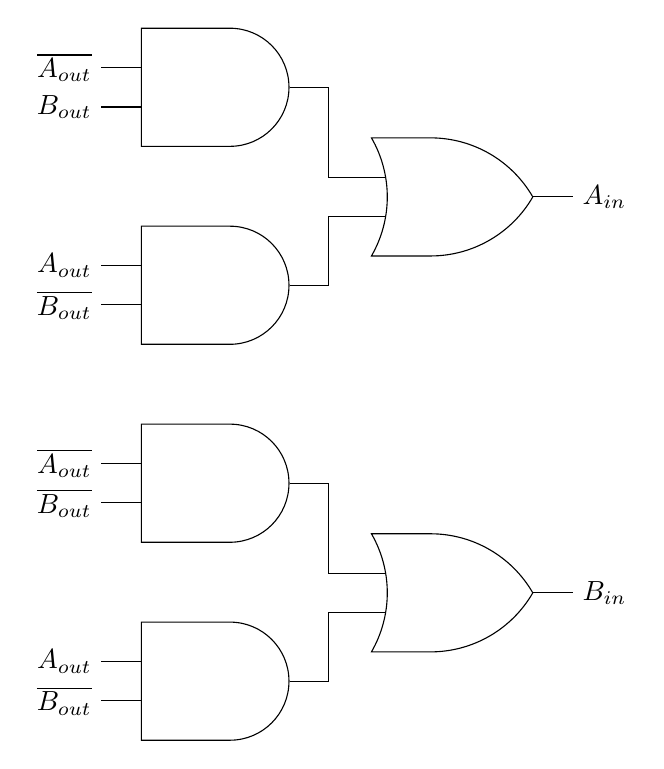
\begin{tikzpicture}[gate/.style={minimum size=1.5cm}]
    \node (and1) [draw,and gate US,logic gate inputs=nn,gate] at (0,0) {};
    \node (and2) [draw,and gate US,logic gate inputs=nn,below=of and1,gate] {};
    \node (and3) [draw,and gate US,logic gate inputs=nn,below=of and2,gate] {};
    \node (and4) [draw,and gate US,logic gate inputs=nn,below=of and3,gate] {};
    \node (or1) [draw,or gate US,logic gate inputs=nn,below right=0.1cm and 1.25cm of and1,gate] {};
    \node (or2) [draw,or gate US,logic gate inputs=nn,below right=0.1cm and 1.25cm of and3,gate] {};
    \draw ($(and1.input 1)-(0.5cm,0)$) -- (and1.input 1) node [left=0.5cm] {\(\overline{A_{out}}\)};
    \draw ($(and1.input 2)-(0.5cm,0)$) -- (and1.input 2) node [left=0.5cm] {\(B_{out}\)};
    \draw ($(and2.input 1)-(0.5cm,0)$) -- (and2.input 1) node [left=0.5cm] {\(A_{out}\)};
    \draw ($(and2.input 2)-(0.5cm,0)$) -- (and2.input 2) node [left=0.5cm] {\(\overline{B_{out}}\)};
    \draw ($(and3.input 1)-(0.5cm,0)$) -- (and3.input 1) node [left=0.5cm] {\(\overline{A_{out}}\)};
    \draw ($(and3.input 2)-(0.5cm,0)$) -- (and3.input 2) node [left=0.5cm] {\(\overline{B_{out}}\)};
    \draw ($(and4.input 1)-(0.5cm,0)$) -- (and4.input 1) node [left=0.5cm] {\(A_{out}\)};
    \draw ($(and4.input 2)-(0.5cm,0)$) -- (and4.input 2) node [left=0.5cm] {\(\overline{B_{out}}\)};
    \draw (and1.output) -- ($(and1.output)+(0.5cm,0)$) |- (or1.input 1);
    \draw (and2.output) -- ($(and2.output)+(0.5cm,0)$) |- (or1.input 2);
    \draw (and3.output) -- ($(and3.output)+(0.5cm,0)$) |- (or2.input 1);
    \draw (and4.output) -- ($(and4.output)+(0.5cm,0)$) |- (or2.input 2);
    \draw (or1.output) -- ($(or1.output)+(0.5cm,0)$) node [right] {\(A_{in}\)};
    \draw (or2.output) -- ($(or2.output)+(0.5cm,0)$) node [right] {\(B_{in}\)};
  \end{tikzpicture}
\end{center}

\bigskip

This answer is acceptable; however, there is a simpler solution:
\begin{gather*}
  A_{in}=A_{out}\oplus B_{out} \\
  B_{in}=\overline{B_{out}}
\end{gather*}

This can be surmised directly from the truth table.  Also, using the information is section 1.3 of the text:
\begin{align*}
  B_{in} &= \overline{A_{out}}\,\overline{B_{out}}+A_{out}\overline{B_{out}} \\
  &= \overline{B_{out}}(\overline{A_{out}}+A_{out}) \\
  &= \overline{B_{out}}(T) \\
  &= \overline{B_{out}}
\end{align*}

The simplified circuits are as follows:

\bigskip

\begin{center}
  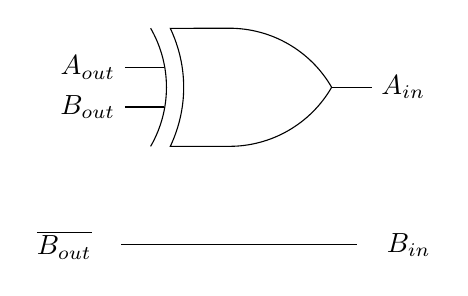
\begin{tikzpicture}[gate/.style={minimum size=1.5cm}]
    \node (xor) [draw,xor gate US,logic gate inputs=nn,gate] at (0,0) {};
    \draw ($(xor.input 1)-(0.5cm,0)$) -- (xor.input 1) node [left=0.5cm] {\(A_{out}\)};
    \draw ($(xor.input 2)-(0.5cm,0)$) -- (xor.input 2) node [left=0.5cm] {\(B_{out}\)};
    \draw (xor.output) -- ($(xor.output)+(0.5cm,0)$) node [right] {\(A_{in}\)};
    \node [coordinate] (a) at (-1.5cm, -2cm) {};
    \node [coordinate] (b) at (1.5cm, -2cm) {};
    \draw (a) -- (b);
    \node [left=0.25cm of a] {\(\overline{B_{out}}\)};
    \node [right=0.25cm of b] {\(B_{in}\)};
  \end{tikzpicture}
\end{center}

\end{document}
